\documentclass[tikz,border=8pt]{standalone}
\usepackage{amsmath,amssymb}
\usepackage{tikz}
\usepackage{pgfplots}
\usepgfplotslibrary{fillbetween}
\pgfplotsset{compat=1.18}
\begin{document}
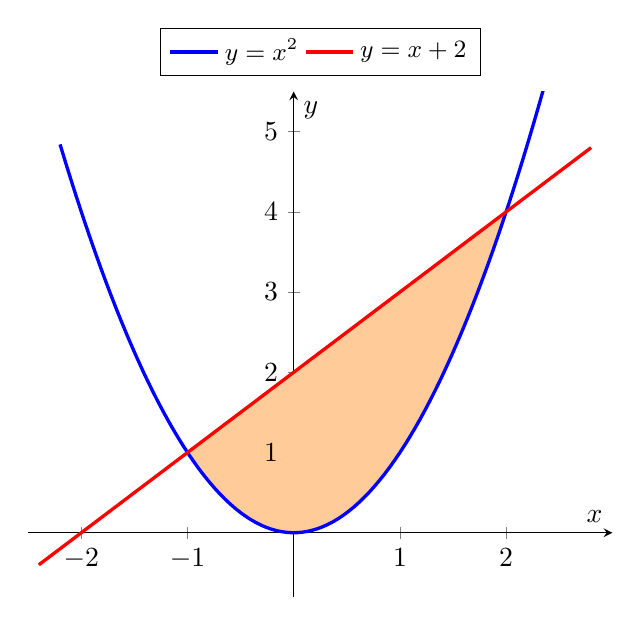
\begin{tikzpicture}
  \begin{axis}[
    axis lines=middle, xlabel={$x$}, ylabel={$y$},
    xmin=-2.5, xmax=3, ymin=-0.8, ymax=5.5,
    xtick={-2,-1,...,2}, ytick={1,...,5},
    width=9cm, height=8cm,
    legend style={font=\small, at={(0.5,1.03)}, anchor=south, legend columns=-1},
  ]
    \addplot[name path=f, very thick, blue, domain=-2.2:2.6, samples=100] {x^2};
    \addlegendentry{$y=x^2$}
    \addplot[name path=g, very thick, red,  domain=-2.4:2.8] {x + 2};
    \addlegendentry{$y=x+2$}
    \addplot[orange!40, forget plot] fill between[of=f and g, soft clip={domain=-1:2}];
  \end{axis}
\end{tikzpicture}
\end{document}
